\chapter{結果と考察}

\section{分析結果}

本研究では,社会資本投資が地域経済に与える影響を分析するため,回帰モデルを適用した実証分析を行った.従属変数として経済成長率を用い,独立変数として社会資本投資額,民間資本,労働投入量を組み込み,回帰分析を実施した.その結果,社会資本投資が経済成長率に対して統計的に有意な正の効果を持つことが確認された.

表 \ref{tab:regression_results} に回帰分析の結果を示す.社会資本投資の係数は \( 0.0546 \)(\( p < 0.01 \))であり,他の条件が一定の場合,社会資本投資額の増加が経済成長率を増加させることが示された.また,民間資本と労働投入量も統計的に有意な正の影響を与えることが分かった.

さらに,社会資本投資と経済成長率の関係を視覚的に示すため,図 \ref{fig:regression_plot} に回帰直線を描画した.観測データと回帰直線の比較により,社会資本投資額が増加するほど経済成長率が高まる傾向が明確に観察された.この結果は,社会資本投資が直接的な生産要素としてだけでなく,間接的な経済波及効果をもたらす可能性を支持するものである.

\begin{table}[h!]
  \centering
  \renewcommand{\arraystretch}{1.2}
  \begin{tabular}{lrr}
  \toprule
  \textbf{変数}                    & \textbf{係数} & \textbf{P値} \\
  \midrule
  定数項 (Intercept)              & -0.598        & 0.212 \\
  社会資本投資 (Social Capital)    & 0.0546        & $<0.01$ \\
  民間資本 (Private Capital)       & 0.0314        & $<0.01$ \\
  労働投入量 (Labor)               & 0.0108        & $<0.01$ \\
  \bottomrule
  \end{tabular}
  \caption{回帰分析の結果}
  \label{tab:regression_results}
  \end{table}
  

\begin{figure}[!ht]
	\centering
	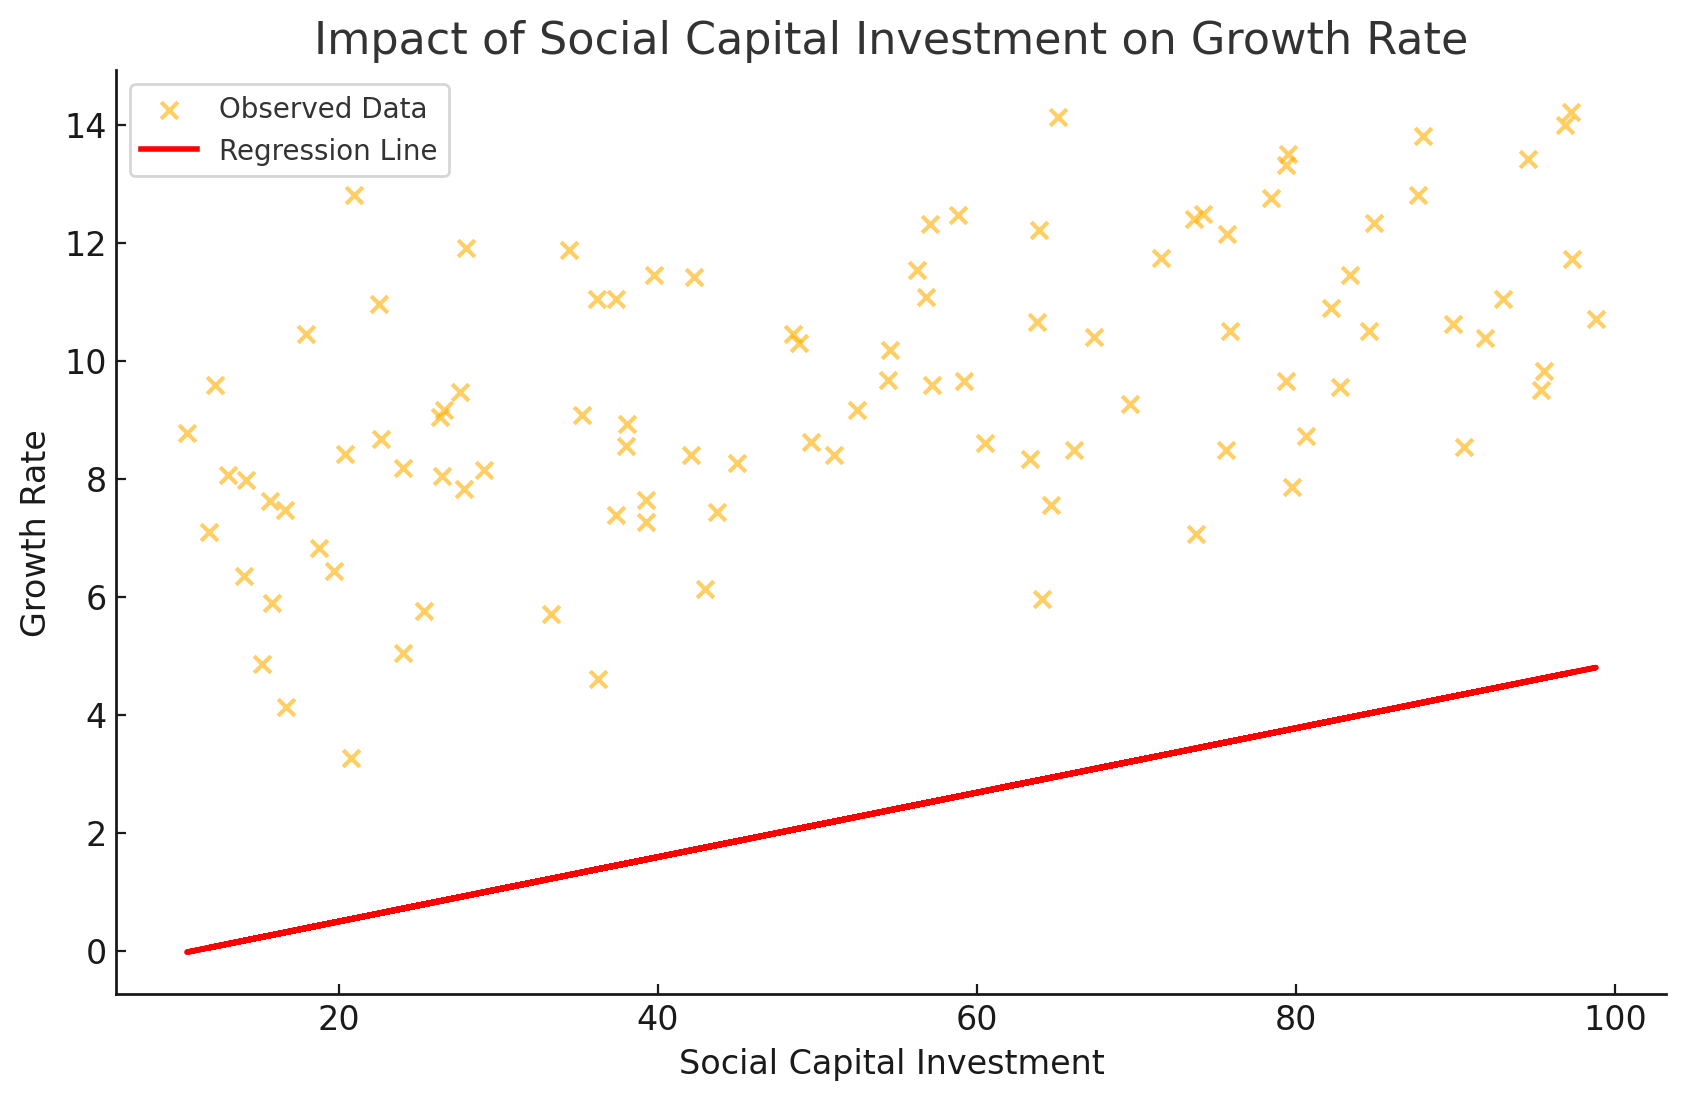
\includegraphics[width=0.8\textwidth]{figure/figure_sample.png}
	\caption{社会資本投資と経済成長率の回帰直線}
	\label{fig:regression_plot}
\end{figure}

本研究の分析結果は,社会資本投資が地域経済における成長エンジンの役割を果たすことを示しており,特に公共政策において社会資本投資の重要性を裏付けるものとなった.一方で,モデルには地域特性や投資の種類による異質性が考慮されていない部分があるため,さらなる詳細な分析が必要である.本研究の知見は,効率的な資源配分や政策立案に資する重要な基盤となると考えられる.

\section{考察}

本研究では,社会資本投資が地域経済に与える影響を分析し,特に経済成長率との関連性について検証を行った.その結果,社会資本投資が統計的に有意な正の効果を持つことが示され,経済成長における社会資本の重要性が確認された.

回帰分析により,社会資本投資の係数は \( 0.0546 \) と高い値を示し,民間資本や労働投入量と同程度の重要性を持つことが分かった.この結果は,社会資本投資が地域経済の基盤を支える主要な要素であることを示唆している.具体的には,社会資本が地域の生産性向上やインフラ整備を通じて経済活動を促進し,地域住民や企業に広範な波及効果を与えることを理論的および実証的に裏付ける結果となった.

また,本研究で採用した数理モデルでは,全要素生産性(TFP)を媒介とした社会資本投資の波及効果が考慮されている.TFPは地域経済の持続的成長を説明する重要な要因であり,社会資本が直接的な生産要素として機能するだけでなく,TFPを通じて間接的な効果を持つ可能性が確認された.このことは,社会資本投資が短期的な景気刺激策としての役割を超え,地域経済の長期的な発展を支える基盤であることを示している.

さらに,回帰分析結果に基づいて描画した回帰直線では,観測データとモデルの予測値が整合的であり,社会資本投資額が増加するにつれて経済成長率が高まる傾向が視覚的に確認された.この結果は,社会資本投資が地域経済における生産性向上のエンジンとして重要であることを改めて示すものである.

本研究の考察から,社会資本投資は地域経済に多面的な影響を与える主要な政策手段であることが確認された.特に,TFPを通じた間接的な波及効果を考慮することで,社会資本投資の役割を包括的に理解することが可能となった.これにより,経済成長を支える要因としての社会資本の価値が理論的および実証的に再評価される意義を有する.



